\documentclass[10pt]{beamer}

\usetheme[progressbar=frametitle]{metropolis}
\usepackage{appendixnumberbeamer}

\usepackage{booktabs}
\usepackage[scale=2]{ccicons}
\usepackage{pgfpages}



\usepackage{pgfplots}
\usepgfplotslibrary{dateplot}

\usepackage{xspace}
%\setbeameroption{show notes on second screen=right} 
%\setbeamertemplate{note page}{\pagecolor{yellow!5}\insertnote}

\pgfdeclareimage[width=\paperwidth]{mybackground}{src/futureits.png}
\newcommand{\themename}{\textbf{\textsc{metropolis}}\xspace}
\hypersetup{pdfpagemode=FullScreen}




\title{Adaptive Beamforming for future ITS}
\subtitle{A neural network approach to antenna beam steering for mmWave Systems}
\author{Clifford Beta \and \\Anne Okemwa}
 \date{\today}

 \titlegraphic{\hfill
\includegraphics[height=1.5cm]{src/logo.png}}

\begin{document}

\maketitle
    
\begin{frame}{mmWave Communication Potential}
  \begin{itemize}[<+- | alert@+>]
    \item \huge multi-gigabit-per second communication
    \item \huge very low latency
  \end{itemize}
\end{frame}
{
\usebackgroundtemplate{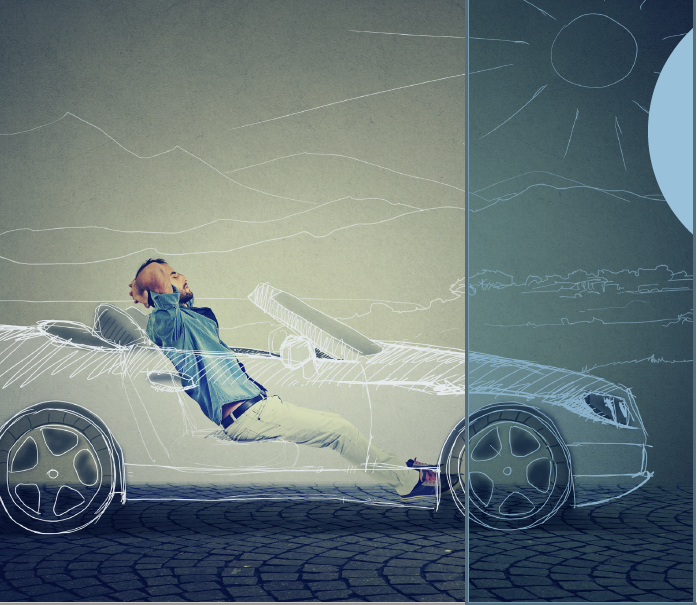
\includegraphics[width=\paperwidth]{src/autonomous.png}}
\begin{frame}{Applications}
  \begin{itemize}[<+- | alert@+>]
    \item \huge Autonomous driving
    \item \huge Immersive gaming
    \item \huge Virtual reality
    \item \huge Augmented reality
  \end{itemize}
\end{frame}
}
\begin{frame}
	\frametitle{Two Figures aside}
	
	\begin{columns}[b]
		\column{0.0125\textwidth}
		\column{0.4875\textwidth}
		\begin{overlayarea}{\textwidth}{.45\textheight}
 		 \only<1-|handout:0>{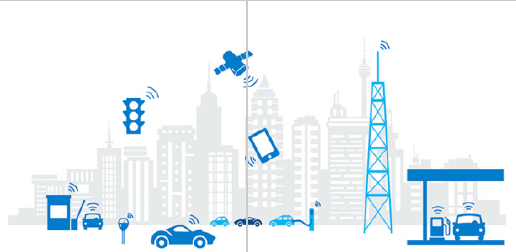
\includegraphics[width=4cm]{src/futureits.png}}
		\end{overlayarea}%
			
		 Be aware, that not every font supports small caps. If for example you typeset your presentation with pdfTeX and the Computer Modern Sans Serif font, every text in smallcaps will be typeset with the Computer Modern Serif font instead.
		
		\column{0.4875\textwidth}
			\begin{overlayarea}{\textwidth}{.45\textheight}
			  \only<2>{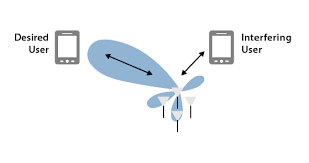
\includegraphics[width=4cm]{src/desired_user.png} }
			\end{overlayarea}
			\par
		Be aware, that not every font supports small caps. If for example you typeset your presentation with pdfTeX and the Computer Modern Sans Serif font, every text in smallcaps will be typeset with the Computer Modern Serif font instead.
		\column{0.0125\textwidth}
		

	\end{columns}
\end{frame}


\begin{frame}[fragile]{Sections}
  Sections group slides of the same topic

  \begin{verbatim}    \section{Elements}\end{verbatim}

  for which \themename provides a nice progress indicator \ldots
\end{frame}

\section{Titleformats}

\begin{frame}{Metropolis titleformats}
	\themename supports 4 different titleformats:
	\begin{itemize}
		\item Regular
		\item \textsc{Smallcaps}
		\item \textsc{allsmallcaps}
		\item ALLCAPS
	\end{itemize}
	They can either be set at once for every title type or individually.
\end{frame}


{\setbeamercolor{palette primary}{fg=black, bg=yellow}
\begin{frame}[standout]
  Questions?
\end{frame}
}

\appendix

\begin{frame}[fragile]{Backup slides}
  Sometimes, it is useful to add slides at the end of your presentation to
  refer to during audience questions.

  The best way to do this is to include the \verb|appendixnumberbeamer|
  package in your preamble and call \verb|\appendix| before your backup slides.

  \themename will automatically turn off slide numbering and progress bars for
  slides in the appendix.
\end{frame}

\begin{frame}[allowframebreaks]{References}

  \bibliography{demo}
  \bibliographystyle{abbrv}

\end{frame}

\end{document}
